\documentclass[journal, a4paper]{IEEEtran}
\usepackage{algorithm}
\usepackage{algpseudocode}
\usepackage{graphicx}
\usepackage{url}  
\usepackage{amsmath}
\usepackage{hyperref}
\usepackage{xcolor}
\graphicspath{ {img/} }
\hypersetup{
  colorlinks=true,
  linkcolor=blue!50!red,
  urlcolor=blue!70!black
}
\begin{document}
\title{C++ Project - Solving Kakuro}
\author{
    Elie ABI HANNA DAHER and Bilal EL CHAMI \\ 
    GitHub repository: \href{https://github.com/elieahd/kakuro}{github.com/elieahd/kakuro}
}
\markboth{Paris Dauphine University}{}
\maketitle
\begin{abstract}
    This document illustrate the work done for an academic project that consists of solving a Kakuro Grid as a contraint satisfaction problem (CSP) in C++.
\end{abstract}
\section{Introduction}
 Kakuro consists in filling a grid with numbers that sum up to a certain values for each column and row. Each cell has a domain of values.\\
 The following example represents a 5x5 grid where the sum of each row has to be 15 as well as the sum of each column.
\begin{figure}[h!]
         \begin{center}
        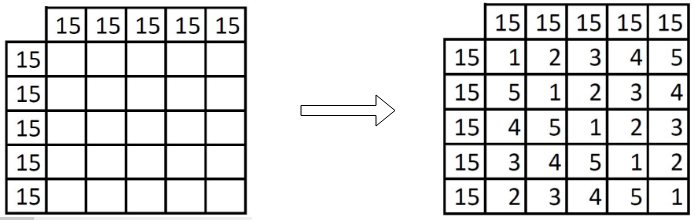
\includegraphics[width=\columnwidth]{example_kakuro.png}
        \caption{Example of solving a 5x5 kakuro gird}
        \label{fig:example_kakuro}
         \end{center}
\end{figure}
\section{Implementation}
In our project we created 4 classes: $Position$, $Cell$, $Grid$ and $Kakuro$.
The $Cell$ class is represented by a value and a $Position$. 
The $Grid$ contain a list of $Cell$. 
Finally the $Kakuro$ contains the $Grid$ with all the possible values that 
a $Cell$ can have as well as the target sum of rows and columns. 
$Kakuro$ class also contains the implemented algorithm: Forward Checking, 
Iterative Sampling and Iterative Meta Monte Carlo. \\
\subsection{Grid}
The initial grid of the kakuro will be present in a file, which will contain the
cell's possible values and it's target sum of each column and row.
We have tested our project in 5 different grids with different sizes between 2x2
 and 6x6 grid. You can find the different girds under the folder \textit{grids} 
 in the GitHub repository.
\subsection{Choosing variable}
While solving the Kakuro grid, we have decided to choose the variable (Cell) 
that has the smallest domain size. 
In both algorithm, forward checking and Monte-Carlo, we implemented the same 
logic regarding the choice of the unassigned variables.
\section{Search Algorithms}
We implemented two algorithms: Forward Checking and Monte-Carlo.
\subsection{Forward Checking}
This algorithm consists in reducing the domain of each unassigned variable. 
Each time a value is assigned to a cell, it is removed from the domain of each 
cell in the same row and column. To check if we need to backtrack, 
two conditions are evaluated, the first one is making sure that all the 
unassigned Cell still have values in their domains then checking that the grid
 is consistent by respecting the sum constraints of each row and column.
\subsection{Iterative Sampling}
This algorithm consists in assigning a random value for a Cell, and in case of inconsistency in the grid or in case of an empty domain for an unassigned cell we will reinitialize the grid and restart the algorithm. 
\subsection{Iterative Meta Monte Carlo}
This algorithm consists in trying all possible values of a Cell, and for each value a sample score will be evaluated then the value that have the lower score will be chosen. 
\section{Experimentals - Simulation}
In order to test the performance of our algorithms, we ran several grids 100 time each and calculated the estimated time to solve the puzzle using all algorithms. \\
    \begin{table}[!hbt]
        \begin{center}
        \caption{Simulation}
        \label{tab:simParameters}
        \begin{tabular}{|c|c|c|c|}
            \hline
           Grids & Forward Checking &  Iterative Sampling & Meta Monte Carlo \\
            \hline
           2x2 & $0.02$ s  &  $ 0.019 $ s   &  $ 0.016 $ s  \\
            \hline
           3x3 & $0.026$ s  &  $ 0.038 $ s &  $ 0.027 $ s    \\
            \hline
           4x4 & $ 0.028  $ s  &  $ 0.488 $ s  &  $ 0.029 $ s   \\
            \hline
           5x5 & $ 0.03 $ s  &  $ 3.598 $ s &  $ 0.045s $ s    \\
            \hline
        \end{tabular}
        \end{center}
    \end{table}

The time of execution of all algorithms depend both on  the size of the grid, the target sum and their possible values.
The forward checking algorithm is more optimal and efficient than Monte-Carlo.\\
\begin{thebibliography}{5}
    \bibitem{MonteCarloKakuro} 
    T.~Cazenave. {\em Monte-Carlo Kakuro}
   \bibitem{WikiKakuro} 
   Wikipedia page on {\em Kakuro}. [Online]. \\ Available:  \url{ https://en.wikipedia.org/wiki/Kakuro}
   \bibitem{WikiCSP} 
   Wikipedia page on {\em CSP }. [Online]. \\ Available:  \url{https://en.wikipedia.org/wiki/Constraint_satisfaction_problem}
   \bibitem{WikiBacktracking} 
   Wikipedia page on {\em Backtracking algorithm}. [Online]. \\ Available:  \url{https://en.wikipedia.org/wiki/Look-ahead_(backtracking)}
\end{thebibliography}
\end{document}


